\chapter{Testing, Interpretation and Evaluation}
\label{cha:tande}
 
Testing the results at all stages of development was done using trial and improvement. As there are no maps publicly available that are doing similar things to Inhale, it was hard to know when I made the correct decision. At most decision points, I didn't know if there was a correct or incorrect decision, just decisions that guided the project in roughly the right direction. That doesn't mean that my decisions were just wild stabs in the dark, they were guided by allergy research. The following resources really helped me make the bulk of my major decisions \cite{childhood, rhinitis, co2pollen, waldo}.\\
 
When the project came together at the end, I noticed a few areas that were indicated as hotspots that you might not expect to have been indicated.

\section{Allergy Hotspots}

In this section I'll go into some detail about the interesting places I found using the final allergy symptom map.

\subsection{Redcar}

Redcar is a small town on the East coast of England with a population of 35,000 \cite{redcarpop}. Large cities tend to have a higher densities of sever allergy symptoms, so it's quite surprising that Redcar is presented as a hotspot as seen in Figure \ref{fig:redcar}.\\

\begin{figure}[H]
\begin{center}
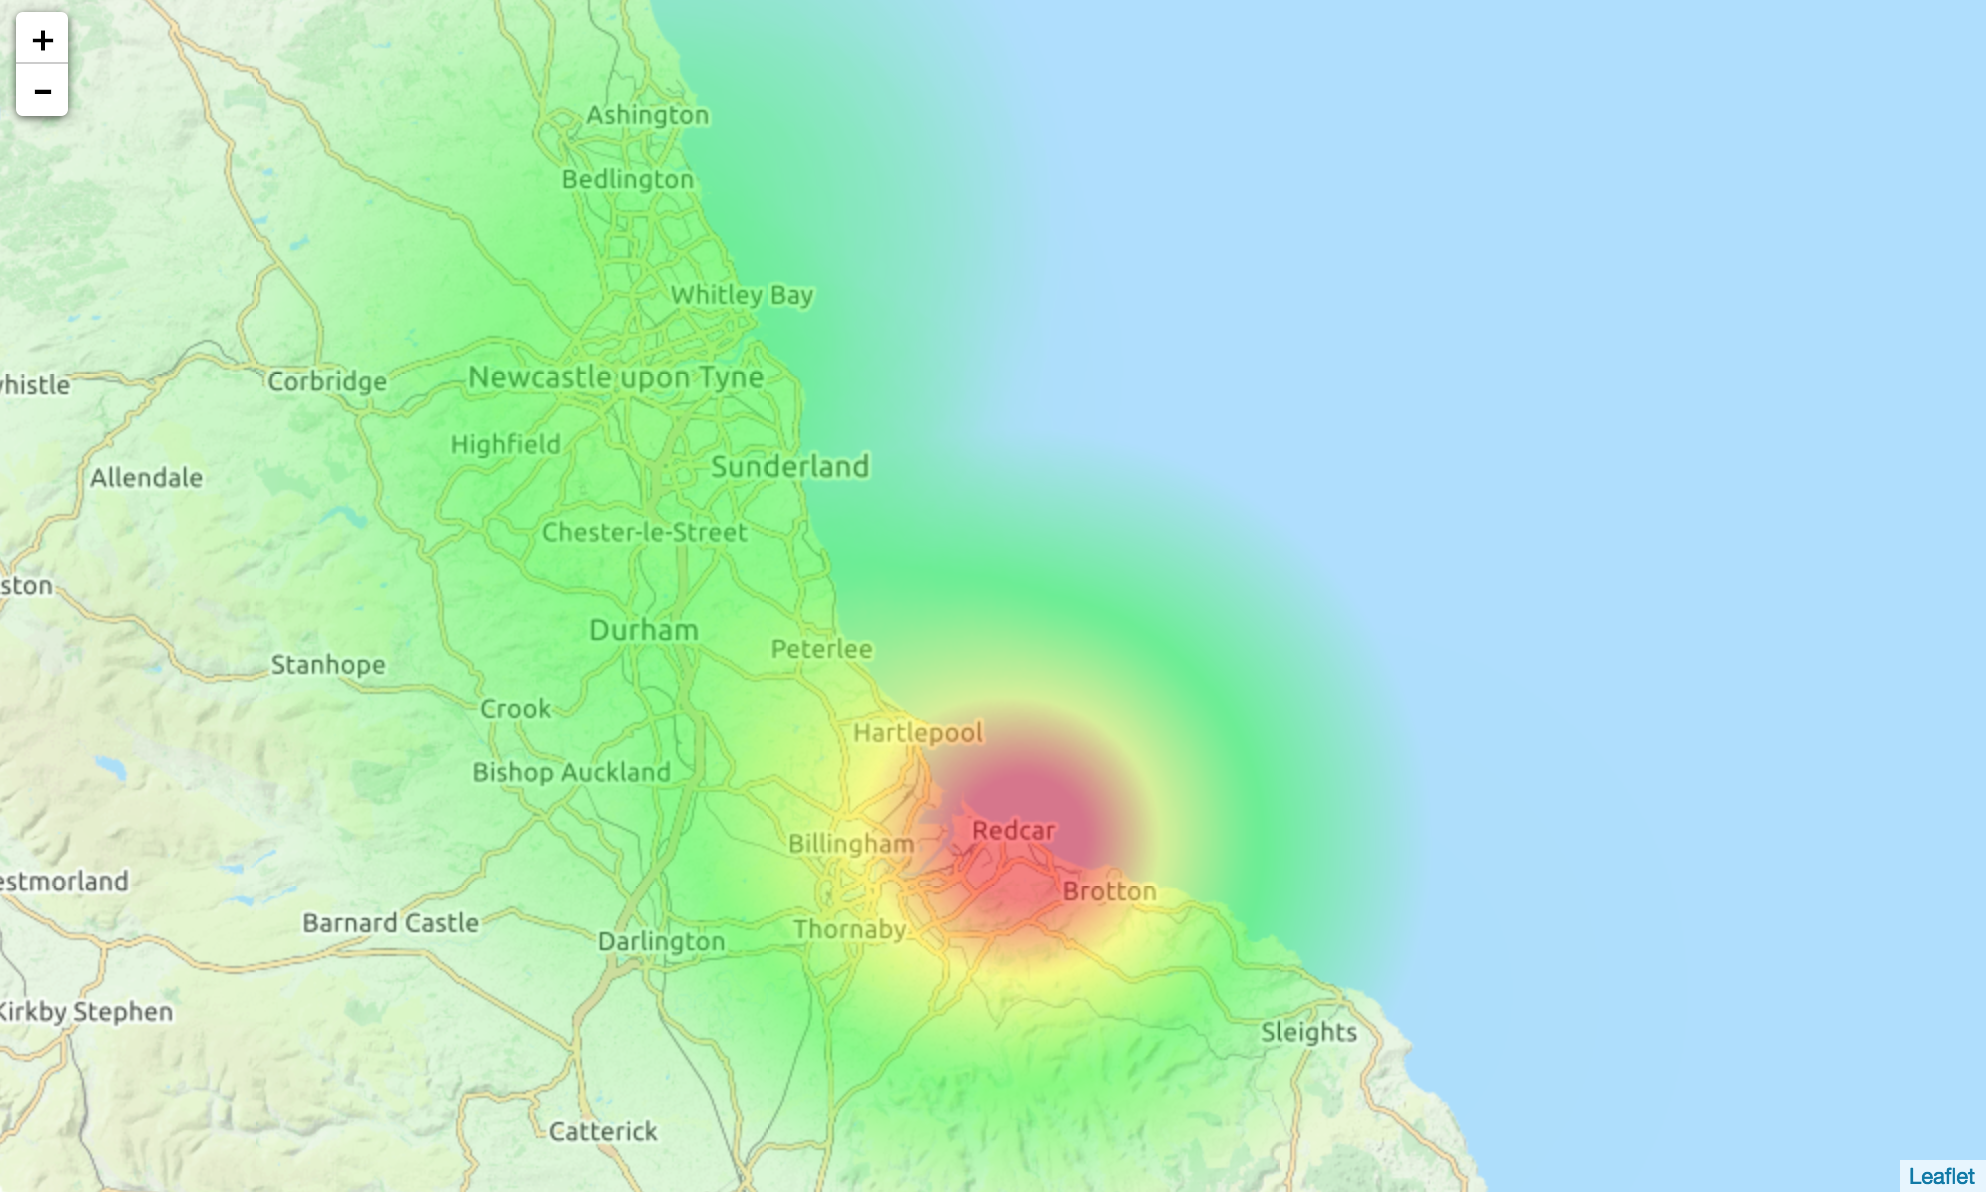
\includegraphics[width=0.6\textwidth]{redcar}
\caption{Redcar, North East England}
\label{fig:redcar}
\end{center}
\end{figure}

I looked into the history of Redcar and I found that until late 2015, Redcar had a large steel industry producing 3.4 million tonnes of steel per year. With a combined directly related job count of 2000, it was a large part of Redcar \cite{bbcredcar}. The Steel industry had been active in Redcar since 1917 meaning that local residents will have been exposed to harsh pollutants for most of their lives. Redcar also has a medium sized car parts plant owned by ElringKlinger, a large German company turning over just under €1B a year \cite{guardez}.\\

The Britain Breathing data given to me is a dump from the month of September 2016. Even though my data is from a year after the steel works has been shutdown, the effects from the steel industry continues to effect the health of residents. Long term exposure to harsh air pollutants can cause permanent health effects \cite{longterm}. So it is quite likely that Redcar's industry, in particular the steel industry is at least partly to explain for the unusually high density of allergy suffers.\\

\subsection{Honourable mention}

Exeter was another surprise hotspot area. With a population of 127,000, it's not exactly a small town but it is highlighted as reasonably high density area of allergy symptoms, even when compared to London and Bristol.\\

\begin{figure}[H]
\begin{center}
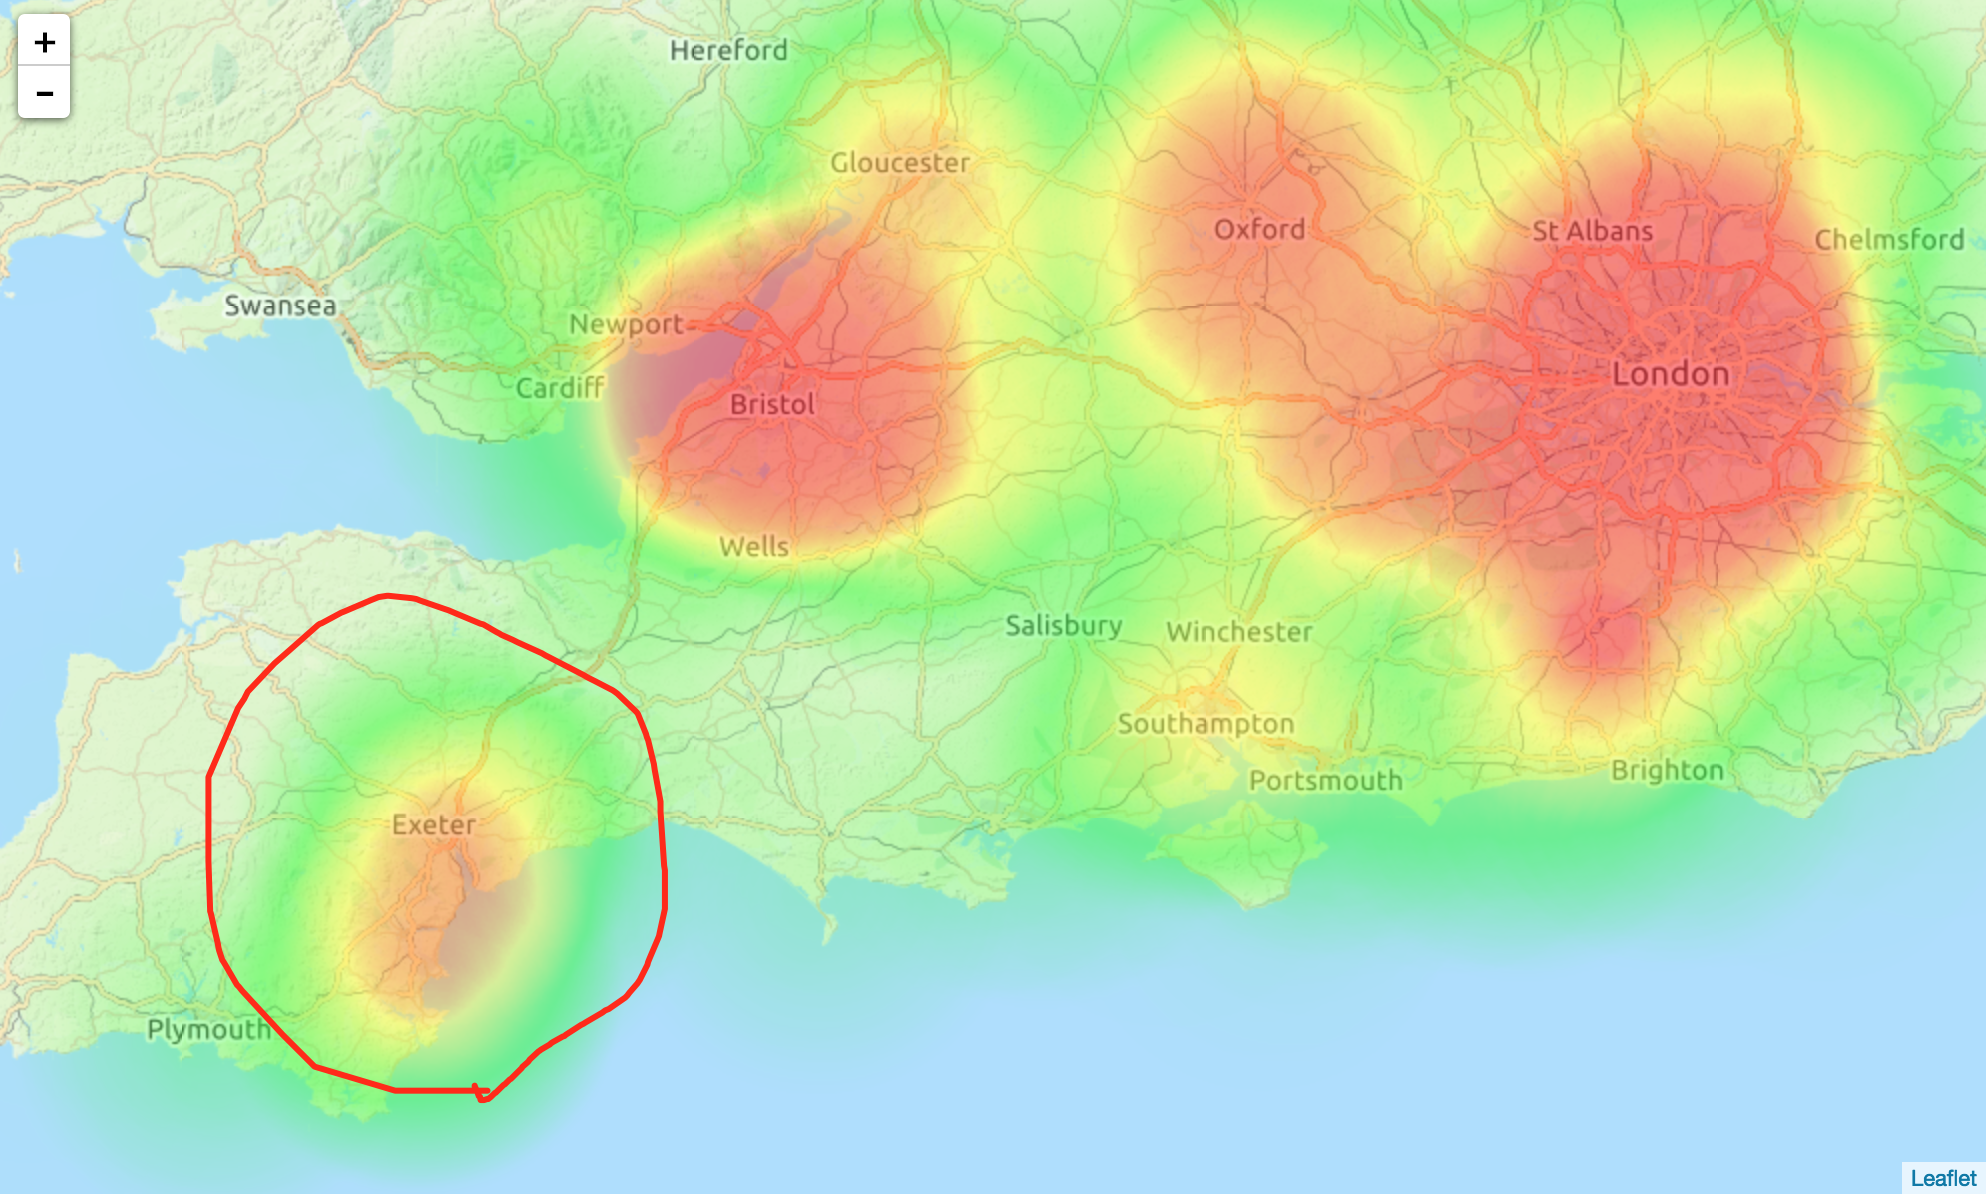
\includegraphics[width=0.6\textwidth]{exeter}
\label{fig:exeter}
\caption{Exeter, South West England}
\end{center}
\end{figure}

Exeter does not have any notably large industry, nothing that could be reasonably linked to allergies. However, since the Romans left Exeter has thrived from its agricultural produce with a strong heritage of farming in the community \cite{oldexeter}.\\

The City of Exeter has a thriving bee community with around 100,000 bees in man made enclosures in the city itself with lots of small bee caring communities in the surrounding areas \cite{beeproj}. Bees need high pollen count crops like oilseed rape to produce honey. Whilst I could not find any hard evidence of Exeter having a larger than average yield for oilseed rape, it's a reasonable suggestion.

\section{Road Traffic Findings}

Before displaying the Road Traffic data on the map, I had hoped that there would be a correlation between allergies and the volume of traffic on the roads. I was quite wrong, there is no real evidence using my presented data that there is a correlation between road traffic and allergy symptoms.\\

I found a good example in the north of England. With the map focused somewhere between Redcar on the west coast and Lancaster on the east coast, you get a good view of the east and west traffic corridors. Look at Figure \ref{fig:rtcor}, you can see there is clearly high levels of pollution from road vehicles on both sides of the country. There is however, not a single hotspot that lies on those roads. The east coast corridor doesn't even show up as a minor hotspot. Looking at the raw data, it's actually one of the better places in the UK to live for allergy symptoms, yet has some of the highest traffic volumes in the area.\\